\chapter{Implementierung}

\section{Struktur des Projekts}
Die Struktur des Projekts auf Datei-Ebene im Ordner \emph{Management} ist folgender
Maßen aufgebaut:

\begin{singlespacing}
	\begin{itemize}
		\item Im Unterordner \emph{Admin} liegen alle Dateien für den Admin-Bereich
		\item Im Unterordner \emph{Frameworks} liegen alle Frameworks die im Projekt verwendet werden
		\item Im Unterordner \emph{Images} liegen alle Bilder und Icons die im Projekt verwendet werden 
		\item Im Unterordner \emph{User} liegen alle Dateien des User-Bereiches
		\item Im Ordner \emph{Management} selbst liegt die \emph{generalConfig.php} Datei, die
		globale Variablen anlegt welche Pfade oder Informationen über die Datenbank
		definiert
	\end{itemize}
\end{singlespacing}


\section{Admin-Bereich}
Der Admin-Bereich ist die Oberfläche über die der Dozent die Möglichkeit hat
neue Fragen, Kategorien, Vorlesungen und Arbeitsblätter zu erstellen.



\subsection{Struktur der Implementierung}
Die Struktur des Admin Bereichs auf Datei-Ebene im Ordner \emph{Admin} ist
folgender Maßen aufgebaut:

\begin{singlespacing}
	\begin{itemize}
		\item Im Unterordner \emph{adminStyles} liegen alle CSS Dateien für den Admin-Bereich
		\item Im Unterordner \emph{js} liegen alle JavaScript Dateien und Bibliotheken für den
		Admin-Bereich
		\item Im Ordner \emph{Admin} selbst liegen alle \gls{PHP} Dateien der einzelnen Unterseiten 
		des Admin-Bereichs
	\end{itemize}
\end{singlespacing}


Die Struktur des Admin Bereichs auf Code-Ebene kann unter dem Begriff der
"`prozeduralen Programmierung"' zusammengefasst werden. Wo dies sinnvoll war, wurden dabei
Funktionen geschrieben die bestimmte Aufgaben abdecken. Durch eine starke
Verzahnung von \gls{PHP} und \gls{HTML} Code und um die Übersichtlichkeit zu gewährleisten, wurde
der \gls{HTML} Code größtenteils mit in den \gls{PHP} Code integriert.


\subsection{Eingesetzte Libraries und Frameworks}
Es werden mehrere Frameworks verwendet um die Funktionalität des Admin-Bereichs
zu erhalten.
\begin{singlespacing}
	\begin{itemize}
	  	\item Mit dem Framework \gls{adoDB}\footnote{AdoDB-Projektseite auf Sourceforge: \url{http://adodb.sourceforge.net}} können Verbindungen mit Datenbank erstellt und gemanaged. Außerdem
			stellt es Funktionen für \gls{SQL} Querys zur Verfügung.
		\item Die bekannte Bibliothek \gls{jQuery}\footnote{JQuery-Projektseite: \url{http://jquery.com}} wird im Admin-Bereich zur Sicherstellung der Crossbrowser-Funktionalität eingesetzt.
		\item Die Bibliothek \gls{PHPQRCode}\footnote{PHPQRCode-Projektseite auf Sourceforge: \url{http://phpqrcode.sourceforge.net}} wird dazu verwendet um QR-Codes durch \gls{PHP} zu
			generieren.
		\item Die Bibliothek \gls{pChart}\footnote{pChart-Projektseite auf Sourceforge: \url{http://pchart.sourceforge.net}} wird zum Erstellen von Auswertungsdiagrammen verwendet.
	\end{itemize}
\end{singlespacing}
 


\subsection{Besonderheiten der Implementierung}
Im Folgenden sollen einige Besonderheiten der Implementierung dargestellt und
erläutert werden.
\begin{singlespacing}
	\begin{itemize}
		\item Damit die Webseite nicht bei jedem Seitenwechsel in der Navigationsleiste
			neu geladen werden muss, wurde zur Navigation Ajax verwendet. Dadurch wird immer
			nur der Seitenbereich mit neuem Content aktualisiert, der Rest der Seite muss
			deswegen nicht unnötig nach geladen werden.
		\item Der QR-Code wird mit der \gls{PHPQRCode} Bibliothek generiert. Dabei ist
			jedoch eine Besonderheit zu beachten: Da der QR-Code nicht unnötig
			zwischengespeichert werden sollte, musste ein besonderes Konstrukt verwendet
			werden. Dabei wird durch eine seperate \gls{PHP} Datei der QR-Code erzeugt und in
			dieser Datei gleichzeitig der Content-Type auf \emph{image/png} gesetzt.
			Anschliesend wird diese \gls{PHP} Datei mit dem generierten Bild in den Image-Tag
			einer anderen Seite eingebettet.
		\item Zur Auswertung von Aufzählaufgaben wird versucht eine möglichst genaue
			Korrektheitsüberprüfung durchzuführen. Dazu werden die gegebenen Antworten der
			Studenten in Kleinbuchstaben konvertiert, Umlaute durch (ae, ue, oe, ss) ersetzt
			und bestimmte Sonderzeichen entfernt. Danach werden diese Antworten mit der nach
			den selben Methoden konvertierten Musterlösung verglichen.
		\item Nach Abschluss des Auswertungsvorganges werden die zu einer Frage
			gehörenden Studentenantworten in einem Diagramm, welches mit der Bibliothek
			\gls{pChart} erstellt wird, dargestellt. In diesem Diagramm sind die Antworten
			grafisch dargestellt.
	\end{itemize}
\end{singlespacing}



\section{LeMon-Bereich}
Der \gls{LeMon}-Bereich begrenzt sich auf das Ausfüllen der für \gls{LeMon} angelegte Arbeitsblätter.
\subsection{Struktur der Implementierung}
Um die Implementierung einfach und übersichtlich zu halten, wurde nach dem Stil
dem Konzept der objektorientierten Programmierung vorgegangen.\\
Folgendermaßen wurde dabei die Ordnerstruktur aufgebaut:

\begin{singlespacing}
	\begin{itemize}
		\item Im Unterordner \emph{css} liegen alle CSS Dateien für den \gls{LeMon}-Bereich
		\item Im Unterordner \emph{image} liegen alle Bilder und Icons, die im
			\gls{LeMon}-Bereich verwendet werden
		\item Im Unterordner \emph{include} liegt zum einen eine PHP Datei, welche die
			Datenbankverbindung sicherstellt und zum anderen eine PHP Datei die zentral alle
			verwendeten Klassen aus dem extra Unterordner \emph{Classes} einbindet.
		\item Im Unterordner \emph{js} liegen alle \gls{JavaScript} Dateien und Bibliotheken für den
			\gls{LeMon}-Bereich
		\item Im Ordner \emph{LeMon} selbst liegt die Arbeitsblatt \gls{PHP} Datei, welche das Layout des Arbeitsblattes festlegt.
	\end{itemize}
\end{singlespacing}


\subsection{Eingesetzte Libraries und Frameworks}
Es werden mehrere Frameworks verwendet um die Funktionalität des LeMon-Bereichs
zu erhalten.
\begin{singlespacing}
	\begin{itemize}
		\item Mit dem Framework \gls{Bootstrap}\footnote{Bootstrap-Projektseite:
			\url{http://getbootstrap.com}}, welches \emph{"`das bekannteste Framework zum Entwickeln
			von responsive mobile first Web-Projekten ist"'} \cite{BootstrapDefinition}, wird
			der LeMon-Bereich auf gängigen Mobilgeräten angepasst dargestellt.
		\item Die bekannte Bibliothek \gls{jQuery}\footnote{JQuery-Projektseite:
			\url{http://jquery.com}} wird im Admin-Bereich zur Sicherstellung der
			Crossbrowser-Funktionalität eingesetzt.
	\end{itemize}
\end{singlespacing}

\section{Benutzeroberfläche}
In diesem Abschnitt werden die Aufgaben der unterschiedlichen Oberflächen kurz
erklärt. Es gibt drei Hauptoberflächen: den \emph{Administrationsbereich}, die
\emph{Ansicht für Studenten} und die \emph{Auswertung}.

\subsection{Administrationsbereich}
In diesem Bereich hat der Dozent die Möglichkeit verschiedene administrative
Aufgaben zu tätigen. Dazu zählen die Funktionen \emph{Fragen anlegen und
verwalten}, \emph{Kategorien anlegen und verwalten}, \emph{Vorlesungen anlegen
und verwalten} und \emph{Arbeitsblätter anlegen und verwalten}.
Im folgenden Screenshot ist zu sehen wie der Administrationsbreich aufgebaut
ist. Im Oberen Bereich der Seite gibt es einen Header mit dem Logo der \gls{HDM},
dazu gibt es im unteren Bereich einen Footer in dem es einen Link zur
Webseite der \gls{HDM} gibt. Auf der linken Seite gibt es eine Navigationsbar über
die es möglich ist zu den einzelnen Funktionen zu navigieren. Rechts-mittig ist
der Bereich in dem die einezlenen Unterformulare der Funktionen angezeigt
werden. 

\begin{figure} [!htb]
	\begin{center}
		  \begin{tabular}{@{}r@{}}
			{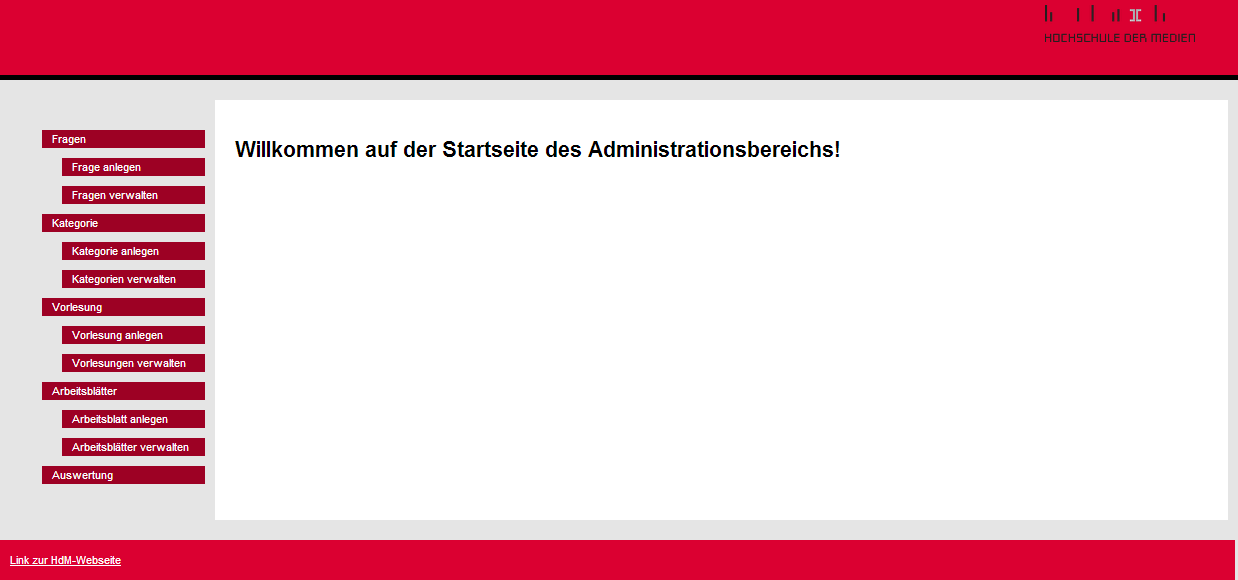
\includegraphics[width=36.6em]{images/Administrationsbereich.png}}\\
 	 	 \end{tabular}
		\caption{Ansicht des Administrationsbereiches}
		\label{fig:Administrationsbereich}
	\end{center} 
\end{figure}\FloatBarrier



\subsection{Ansicht für Studenten}
Diesen Bereich bekommen Studenten zu sehen, wenn sie Aufgabenblätter bearbeiten
sollen. Es werden hier die Fragen für ein bestimmtes Arbeitsblatt aufgelistet.
Die Studenten können das Ausgabenblatt ausfüllen und das Formular abschicken
oder alle Eingabefelder leeren.

\begin{figure} [!htb]
	\begin{center}
		  \begin{tabular}{@{}r@{}}
			{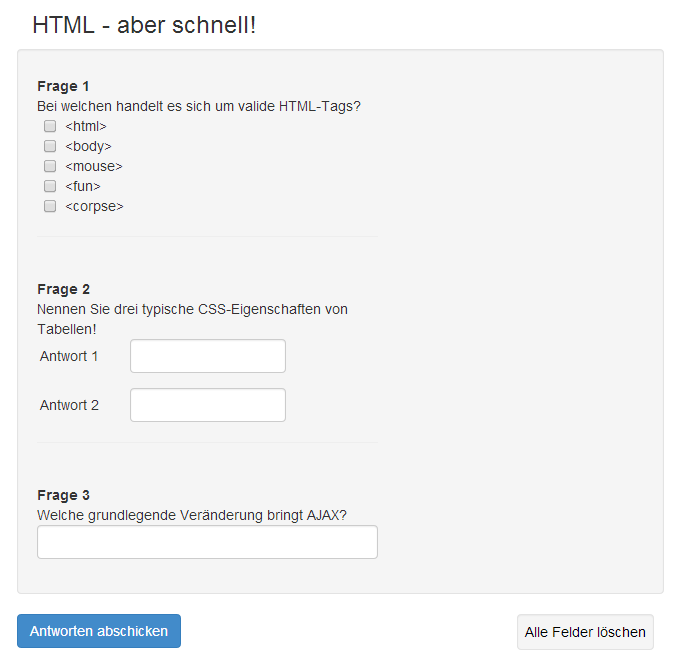
\includegraphics[width=36.6em]{images/Studentenansicht.png}}\\ 
 	 	 \end{tabular}
		\caption{Ansicht für Studenten}
		\label{fig:Studentenansicht}
	\end{center} 
\end{figure}\FloatBarrier

\subsection{Auswertung}
In dem Bereich der Auswertung werden zu einer ausgewählten Vorlesung und einem
Arbeitsblatt die dazugehörigen beantworteten Fragen in Diagrammen oder
Textfelder dargestellt.

\begin{figure} [!htb]
	\begin{center}
		  \begin{tabular}{@{}r@{}}
			{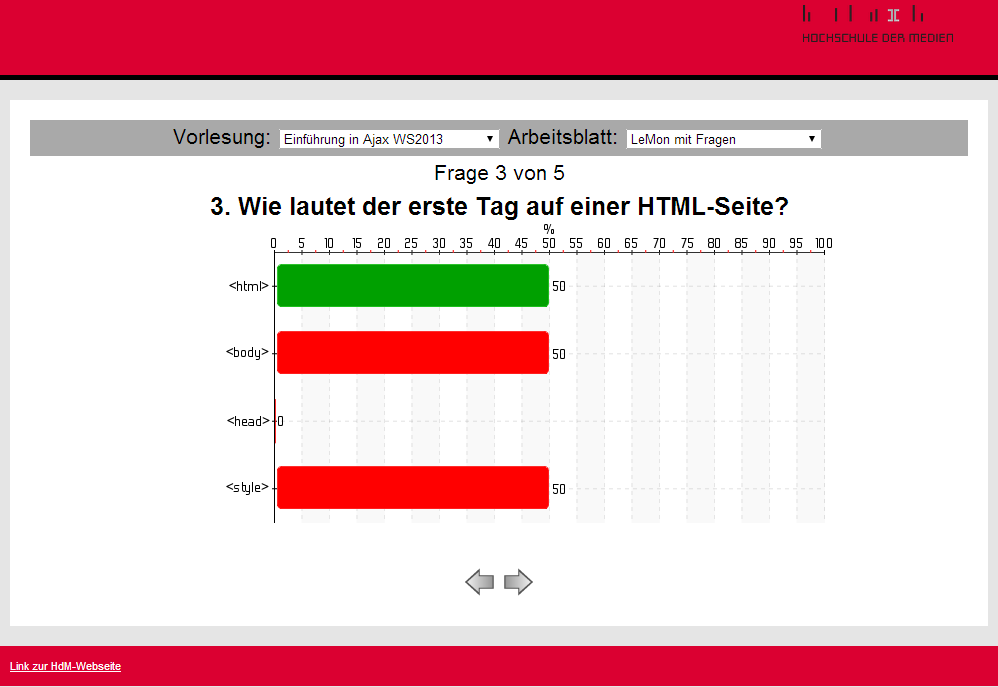
\includegraphics[width=36.6em]{images/Auswertung.png}}\\
 	 	 \end{tabular}
		\caption{Ansicht der Auswertung}
		\label{fig:Auswertung}
	\end{center} 
\end{figure}\FloatBarrier

